\documentclass[12pt]{article}
\usepackage[utf8]{inputenc}
\usepackage{amssymb,tikz-cd,amsmath,amsthm,enumitem}
\usepackage{color}
\usepackage{tikz}
\usetikzlibrary{shapes.misc,calc,math}
\usetikzlibrary{shapes}
\usetikzlibrary{external}
\tikzset{
vtx/.style={inner sep=2.1pt, outer sep=0pt, circle, fill=blue!50!white,draw=black},
vtx2/.style={inner sep=2.1pt, outer sep=0pt, circle, fill=red!50!white,draw=black},
vtx4/.style={inner sep=3.5pt, outer sep=0pt, circle, fill=blue!50!white,draw=black},
triangle/.style={fill=pink,opacity=0.5,line width=1pt},
novtx/.style={cross out, draw=red, line width=2pt},
gsvtx/.style={inner sep=2.1pt, outer sep=0pt, rectangle, fill=green!50!white,draw=black},
gs2vtx/.style={inner sep=1.8pt, outer sep=0pt, regular polygon,regular polygon sides=5, fill=red!50!white,draw=black},
gs3vtx/.style={inner sep=1.4pt, outer sep=0pt, diamond, fill=yellow!50!white,draw=black},
gs4vtx/.style={inner sep=3.5pt, outer sep=0pt, rectangle, fill=green!50!white,draw=black},
axisedge/.style={-latex, line width=1.5pt},
}

\begin{document}

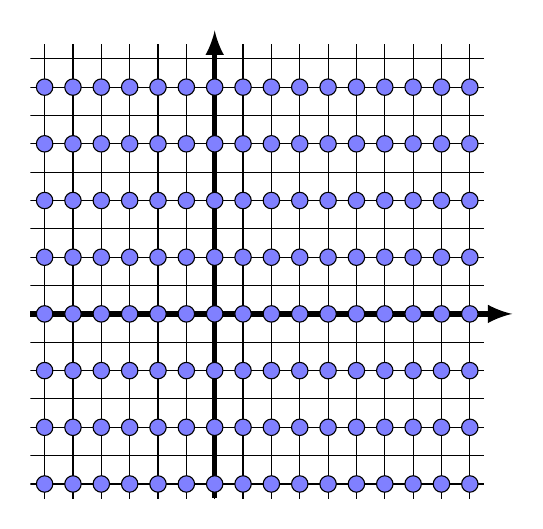
\begin{tikzpicture}[scale=0.36]
\draw[-latex,line width=2pt] (-0.5,6) -- (16.5,6); 
\draw[-latex,line width=2pt] (6,-0.5) -- (6,16); 
\clip (-0.5,-0.5) rectangle (15.5,15.5);
\draw (-1,-1)grid(16,16);
\begin{scope}[xshift=0cm,yshift=0cm]
\foreach \x in {0,...,15}{
\foreach \y in {0,...,8}{
\draw (\x,2*\y)node[vtx]{};
}
}
\end{scope}
\end{tikzpicture}

\end{document}